\documentclass{article}
\usepackage{graphicx}
\usepackage{geometry}


\geometry{
	a4paper,
	total={210mm,297mm},
	left=20mm,
	right=20mm,
	top=20mm,
	bottom=20mm,
}
\begin{document}
	
	\begin{center}
		\textbf{\bfseries\Large ASSIGNMENT NO. 4}
		\\[1cm]
	\end{center}
	
	
	\section{TITLE : } Implementation of 0-1 knapsack problem using branch and bound approach.
	
	\section{OBJECTIVE : }  To study 0-1 knapsack problem using branch and bound approach.
	
	\section{THEORY : }
	
	The knapsack problem or rucksack problem is a problem in combinatorial optimization: Given a set of items, each with a mass and a value, determine the number of each item to include in a collection so that the total weight is less than or equal to a given limit and the total value is as large as possible. It derives its name from the problem faced by someone who is constrained by a fixed-size knapsack and must fill it with the most valuable items.\\
	The most common problem being solved is the 0-1 knapsack problem, which restricts the number xi of copies of each kind of item to zero or one. Given a set of n items numbered from 1 up to n, each with a weight wi and a value vi, along with a maximum weight capacity W.\\
	
	\subsection{MATHEMATICAL MODEL : }
	
	\begin{figure}[h!]
		\centering
		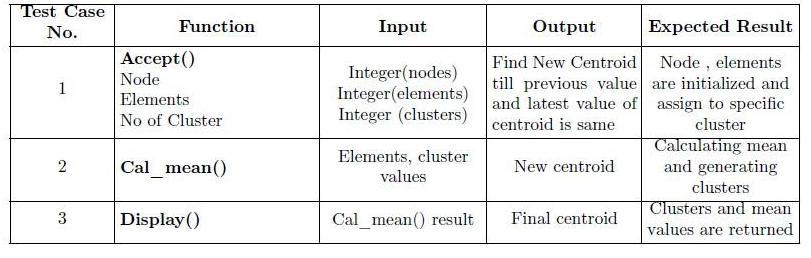
\includegraphics[scale=0.5]{204/5 assign(knapsack)/temp.png}
	\end{figure}
	
	Here xi represents the number of instances of item i to include in the knapsack. Informally, the problem is to maximize the sum of the values of the items in the knapsack so that the sum of the weights is less than or equal to the knapsack's capacity.
	The bounded knapsack problem (BKP) removes the restriction that there is only one of each item, but restricts the number  of copies of each kind of item to an integer value  :\\
	
	\begin{figure}[h!]
		\centering
		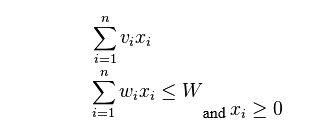
\includegraphics[scale=0.5]{204/5 assign(knapsack)/temp1.png}
	\end{figure}
	
	The unbounded knapsack problem (UKP) places no upper bound on the number of copies of each kind of item and can be formulated as above except for that the only restriction on  is that it is a non-negative integer.\\
	
	
	
	\subsection{ELIMINATION OF REDUNDANT CONTROL STATEMENTS : } We have managed to eliminate redundant control statements by designing proper class in C++
	
	\section{TESTING :}
	
	\subsection{BLACK BOX TESTING : }
	Black-box testing is a method of software testing that examines the\\ function- ability of an application without peering into its internal structures or workings.\\
	This method of test can be applied to virtually every level of\\ software testing:unit, integration, system and acceptance\\
	\textbf{Input :}   Weight and maximum capacity of knapsack\\
	\textbf{Output :} Optimal Solution
	
	
	\subsection{ 0/1 Knapsack problem Using Branch and Bound  }
	Branch and bound is an algorithm design paradigm which is generally used for solving combinatorial optimization problems. These problems typically exponential in terms of time complexity and may require exploring all possible permutations in worst case. Branch and Bound solve these problems relatively quickly.
	
	Let us consider below 0/1 Knapsack problem to understand Branch and Bound.
	
	Given two integer arrays val[0..n-1] and wt[0..n-1] that represent values and weights associated with n items respectively. Find out the maximum value subset of val[] such that sum of the weights of this subset is smaller than or equal to Knapsack capacity W.
	
	Let us explore all approaches for this problem.
	
	A Greedy approach is to pick the items in decreasing order of value per unit weight. The Greedy approach works only for fractional knapsack problem and may not produce correct result for 0/1 knapsack.
	We can use Dynamic Programming (DP) for 0/1 Knapsack problem. In DP, we use a 2D table of size n x W. The DP Solution doesn’t work if item weights are not integers.
	Since DP solution doesn’t alway work, a solution is to use Brute Force. With n items, there are 2n solutions to be generated, check each to see if they satisfy the constraint, save maximum solution that satisfies constraint. This solution can be expressed as tree.
	
	We can use Backtracking to optimize the Brute Force solution. In the tree representation, we can do DFS of tree. If we reach a point where a solution no longer is feasible, there is no need to continue exploring. In the given example, backtracking would be much more effective if we had even more items or a smaller knapsack capacity.i4
	
	
	Branch and Bound
	
	The backtracking based solution works better than brute force by ignoring in feasible solutions. We can do better (than backtracking) if we know the best possible solution sub tree rooted with every node. If the best in sub tree is worse than current best, we can simply ignore this node and its sub trees. So we compute bound (best solution) for every node and compare the bound with current best solution before exploring the node.
	Example bounds used in below diagram are, A down can give $315, B down can $275, C down can $225, D down can $125 and E down can 30.
	
	Branch and bound is very useful technique for searching a solution but in worst case, we need to fully calculate the entire tree. At best, we only need to fully calculate one path through the tree and prune the rest of it.
	
	
	\begin{figure}[h!]
		\centering
		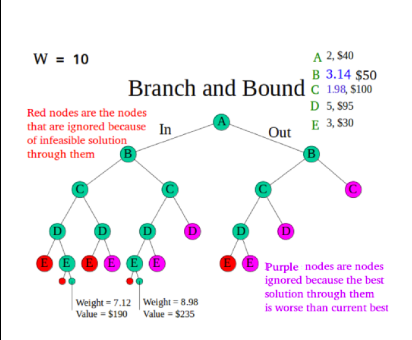
\includegraphics[scale=0.8]{204/5 assign(knapsack)/branchnbound.png}
	\end{figure}
	
	\subsection{WHITE BOX TESTING : }
	White-box testing (also known as clear box testing, glass box testing, transparent box testing, and structural testing) is a method of testing software that tests internal structures or workings of an application, as opposed to its functionality(i.e. black-box testing). While developing 
	test cases for white box testing it is understood that complete testing 
	is impossible. In White Box testing we checkup to which extent the code 
	is being executed, i.e. Covered. There are different kinds of coverage like, statement coverage, path coverage, etc. We will use one of the most popular technique i.e. Statement coverage. Statement coverage is a white box testing technique, which involves the execution of all the statements at least once in the source code. It is a metric, which is used to calculate and measure the number of statements in the source code which have been executed. For this, we will use Flow Graphs. Flow graphs are, Syntactic abstraction of source code Resembling to classical flow charts Forms the basis for white box test case generation principles.Conventions of flow graph notation, \\
	\begin{figure}[h!]
		\centering
		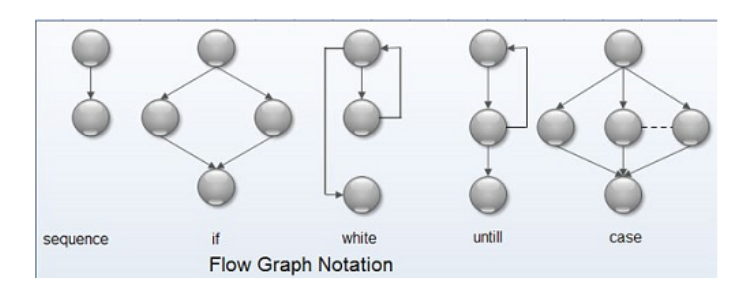
\includegraphics[scale=0.5]{204/5 assign(knapsack)/pqr.png}
	\end{figure}
	
	\subsection{ POSITIVE/NEGATIVE TESTING }
	
	\textbf{Positive Testing :}\\
	To find optimal solution considering all the items
	Example- Input sequence(17) key (17) output(true ,1)\\
	
	\noindent\textbf{ Negative Testing :}\\
	Should fail if wrong data is provided
	
	
	\subsection{ADVANCED TESTING TECHNIQUE}
	Google Testing Framework can be used in future for testing the code
	\section{ Pseudocode: }\\
	\textbf
	1. Sort all items in decreasing order of ratio of value per unit weight so that an upper bound can be computed using Greedy Approach.\\
	2.Initialize maximum profit, maxProfit = 0\\
	3. Create an empty queue, Q.\\
	4. Create a dummy node of decision tree and enqueue it to Q. Profit and weight of dummy node are 0.\\
	5. Do following while Q is not empty.\\
	Extract an item from Q. Let the extracted item be u.\\
	Compute profit of next level node. If the profit is more than maxProfit, then update maxProfit.\\
	Compute bound of next level node. If bound is more than maxProfit, then add next level node to Q.\\
	Consider the case when next level node is not considered as part of solution and add a node to queue with level as next, but\\ 	   Aweight and profit without considering next level nodes.\\
	
	\section{CONCLUSION : }
	
	Hence, we have successfully studied and implemented  0-1 knapsack problem using branch and bound approach.
	
	\begin{center}
		\begin{tabular}{|c|c|c|c|c|}
			\hline	
			•Roll No &  Name of Student & Date of Performance & Date of Submission&Signature of Staff\\ \hline
			•$BECOC357$    & $Sunny  $ $Shah$& 27 / 07 /2017 & 31 / 08 / 2017 \\ \hline
		\end{tabular}•
	\end{center}•
	
	
	
\end{document}


